\chapter{L’exemple des myopathies congénitales et la difficulté du diagnostic}
Dans cette thèse, nous cherchons à développer des méthodes \gls{ia} pour exploiter les données biomédicales. En guise de cas d'application pour développer et évaluer ces méthodes, nous  nous intéressons aux myopathies congénitales, une famille de maladies des muscles rare et génétique dont le diagnostic est complexe. Dans ce chapitre nous allons présenter le contexte biologique de cette maladie avec une présentation de la structure du muscle, de la classification des myopathies congénitales et de leur diagnostic.

\section{Le muscle, un organe particulier assurant des fonctions diverses}
Le muscle est un organe particulier tant par sa structure que son abondance dans le corps humain. Pour un adulte, les muscles représentent près de 40\% de la masse corporelle totale (\cite{janssen_skeletal_2000}). Les muscles assurent une variété de fonction dont le mouvement et la posture, mais aussi la thermogénèse et l'équilibre métabolique.

Dans le muscle, une variété de processus sont nécessaires pour permettre d'assurer ses fonctions. Le muscle intègre des processus neurologiques pour le transfert de signal induisant la contraction. Cette contraction est possible grâce à une structure particulière du muscle en fibres que nous présenterons en détail dans une section suivant. De plus, cette contraction requiert de l'énergie qui est assurée par des processus métaboliques. Enfin le muscle, en raison des contraintes physiques subit lors des mouvements, est un organique dynamique, ainsi des processus assurant la régénération musculaire sont à l'oeuvre pour assurer sa plasticité.

\subsection{Type de muscles}
Il existe dans le corps humains trois types de muscles différents avec des structures différentes en fonction de la fonction qu'ils doivent assurer (figure \ref{fig:muscle-type}, \cite{gomez_oca_physiological_2021}): le muscle lisse, le muscle cardiaque et le muscle strié squelettique.
\begin{figure}[!htbp]
 \centering
 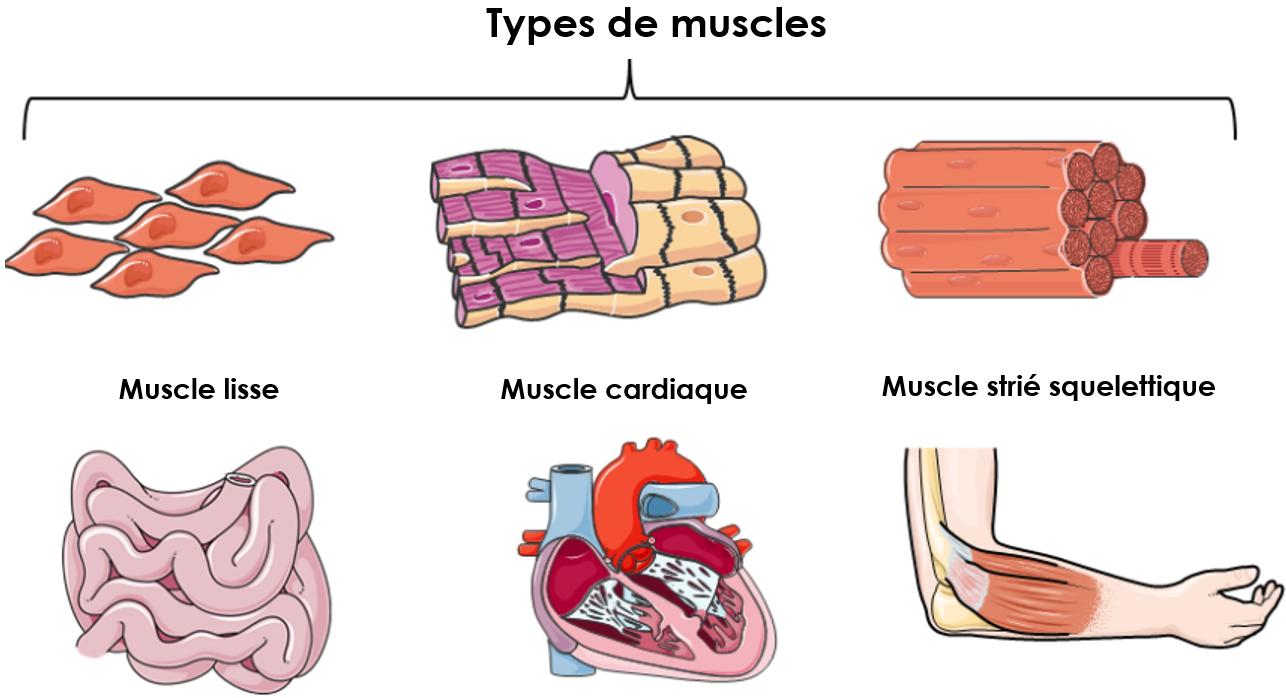
\includegraphics[width=0.8\textwidth]{figures/muscle_type.png}
 \caption[Schéma des trois types de muscles]{Schéma des trois types de muscles (traduit de \cite{gomez_oca_physiological_2021})}
 \label{fig:muscle-type}
\end{figure}
\subsubsection{Muscle lisse}
Le muscle lisse, aussi nommé non-strié, tire son nom de l'absence de striations lors de l'observation au microscope. Les fibres ne possède qu'un seul noyaux central. Ce type de muscles est présent dans les vaisseaux sanguins, l'appareil digestif, l'appareil respiratoire, urinaire et la parois des viscère. La particularité des muscles lisses est qu'ils ne contractent que de manière involontaires, sans contrôle conscient. La contraction de ces muscles est régie par le système nerveux neuro-végétatif (système autonome)

\subsubsection{Muscle strié cardiaque}
Le muscle strié cardiaque est un muscle qui se retrouve exclusivement dans le coeur. Il partage des caractéristiques commune à la foi au muscle lisse et au muscle strié squelettique. Ce muscle se contracte de manière involontaire, et les fibres ne possède qu'un seul noyaux central similairement au muscle lisse. Mais le muscle cardiaque présente des striations similaires au muscle strié squelettique. La caractéristique unique du muscle strié cardiaque est qu'il fonctionne en continu et de se contracter en rythme de façon coordonnée. Ainsi ce muscle est très dépendant du métabolisme oxydatif.

\subsubsection{Muscle strié squelettique}
Enfin les muscles striés squelettiques (nommés communément muscles volontaires) sont les muscles mobilisés lors des mouvements conscient et volontaire, lorsque l'on porte un objet ou que l'on fait du sport. Au miscoscope ces muscles se démarquent par la présence de stries transversales et longitudinales. Ces cellules composants les fibres musculaires du muscle strié squelettique ont la particularité d'avoir fusionner ensembles formant ainsi un "syncitium vrai". Cette fusion donne donc aux fibres musculaires les caractéristiques des cellules géantes (entre 1 et 5 cm de long et 10 à 100µm de diamètre). Ainsi ces cellules osnt multinuclées avec des noyaux périphériques.

Comme leur nom l'indique, ces muscles sont reliés aux os par l'intermédiaire du tendon, leur contraction permet donc le mouvement des os et donc du corps. Cette contraction est engagée sous le contrôle du système nerveux somatique. En fonction de l'intensité et de la durée de la contraction, les muscles striés squelettiques peuvent fonctionner de manière aérobie grâce à leur vascularisation importante ou de façon anaérobie.

Dans le cadre des myopathies congénitales, les muscles striées squelettiques sont affectés et ne sont plus capables d'assurer leur fonction normale en raison d'altérations structurelles, entraînant un déficit de tonus musculaire et de force.

\subsection{Structure du muscle strié squelettique}
Pour comprendre comment les altérations de la structure du muscle qui ont leur lors des myopathies congénitales peuvent mener à son dysfonctionnement, il est important de comprendre comment le muscle est structurer et comment il peut se contracter.

L'organisation du muscle peut être décrite comme celle d'une corde d'escalade. Une corde d'escalade semble être composée d'un seul élément fort et résistant. Mais si l'on regarde de plus près, une corde d'escalade est constituée d'une gaine qui entoure l'âme de la corde. Cette âme est composée de plusieurs gros filaments, eux-même composée de plusieurs filaments de plus en plus fins, torsadés ensemble. 

Ainsi par une métaphore, le muscle entier est comme la corde d'escalade, sa structure est décrite dans la figure \ref{fig:muscle_struct} (\cite{burr_basic_2019}). Le muscle entier entouré par sa gaine nommée \textit{epimysium} est constitué de plusieurs faisceaux musculaire qui le composent. Chacun de ces faisceaux ou fascicules, est composée de filaments encore plus fins nommés fibre musculaire. Ces fasicules et fibres musculaire sont encore observables au microscope optique. Enfin, chacun de ces fibres musculaire est en fait un regroupement de plus petits filaments nommées Myofribrilles qui  sont des filaments composés d'une multitude de myofilaments capables de se contracter. Les myofibrilles et myofilaments ne sont observables qu'en microscopie électronique.

\begin{figure}[!htbp]
 \centering
 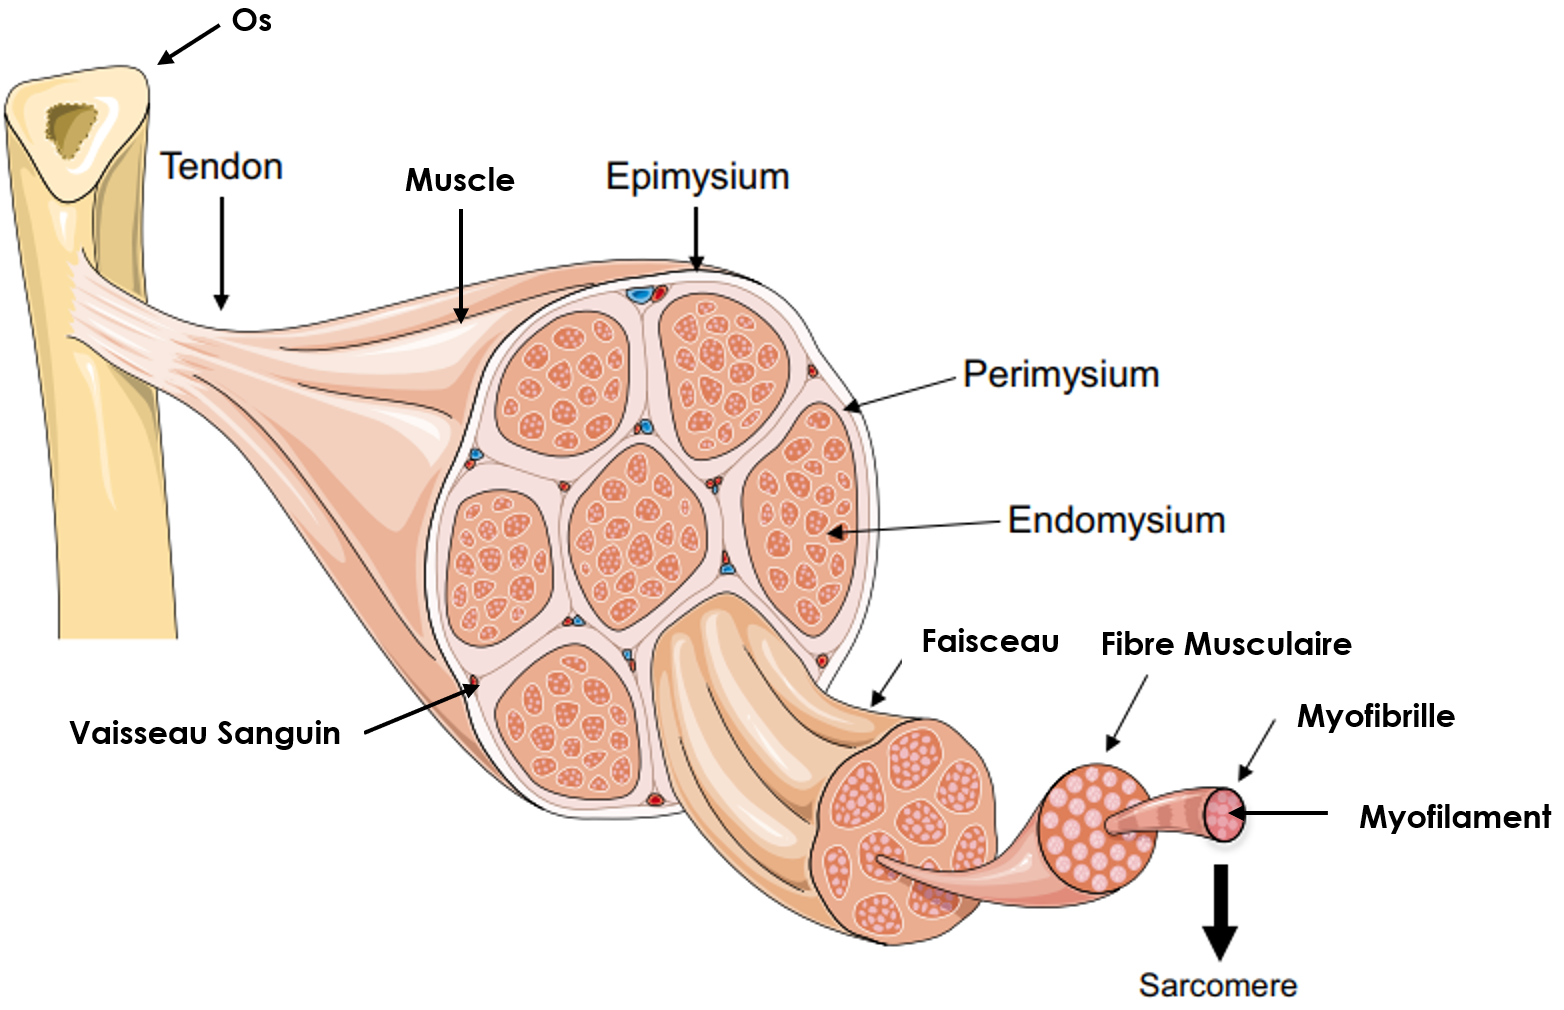
\includegraphics[width=0.8\textwidth]{figures/muscle.png}
 \caption[Schéma de la structure du muscle strié squelettique (modifié de \cite{burr_basic_2019}]{Schéma de la structure du muscle strié squelettique (modifié de \cite{burr_basic_2019}.}
 \label{fig:muscle_struct}
\end{figure}
A une échelle encore plus petite, les myofibrilles sont organisée en plusieurs sarcomère, présentés en figure \ref{fig:sarcomere} (\cite{burr_basic_2019}). Les sarcomères sont l'unité contractile de base des myofibrilles. Il est constitué des trois systèmes de filaments protéïques: (i) un filaments épais de myosine, (ii) un filament mince d'actine inséré sur le disque Z et (iii) un filament élastique enchâssé sur le filament de myosine composé de la titine inséré sur le disque Z aussi.

Lors d'une contraction musculaire les filaments de myosine et d'actine dans la bande A glissent les uns sur les autres, réduisant ainsi la zone H, le muscle est contracté, le sarcomère est raccourcis. On comprend alors qu'un dysfonctionnement dans l'une de trois protéines essentielle à ce mouvement de contraction altère la structure du sarcomère et donc la capacité contractile du muscle. Les gènes TTN, ACTA1 et MYH2/MYH7 (codant respectives pour la titine, actine et myosine) sont des gènes typiquement responsables de myopathies lors qu'ils sont mutés. Cependant nous verrons l'ensemble des gènes responsables des myopathies congénitales dans un section suivante.
\begin{figure}[!htbp]
 \centering
 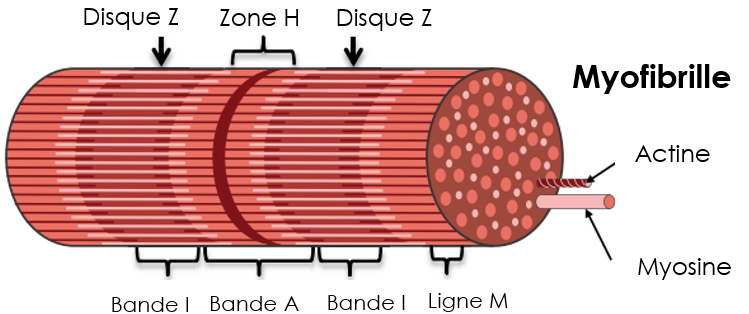
\includegraphics[width=0.8\textwidth]{figures/sarcomere.png}
 \caption[Schéma de la structure du sarcomère.]{Schéma de la structure du sarcomère (modifié de \cite{burr_basic_2019}).}
 \label{fig:sarcomere}
\end{figure}

\subsection{Types de fibres musculaires}
Les fibres musculaires peuvent être classée en trois sous-type de fibres: les fibres de type 1, les fibres de type 2A et 2B qui ont des caractéristiques stucturelles et fonctionnelles différentes. Cette classification repose sur le profil d'expression de la chaine lourde de la myosine. Il existe plusieurs isoforme de la myosine, permettant chacun une contraction plus ou moins rapide et résitante à la fatigue. Le tableau \ref{table:fiber-compare} répertorie les différence principales entre les fibre de type 1, 2B et 2A.

\begin{table}[!htbp]
\centering
\begin{tabular}{|l|c|c|c|} 
 \hline
 \textbf{Caractéristique} & \textbf{Fibre Type 1} & \textbf{Fibre Type 2B}  & \textbf{Fibre Type 2A} \\
 \hline
Couleur & Rouge & Pâle & Pâle \\
Vitesse de Contraction & Lente & Rapide & Rapide \\
Voie métabolique & Aérobie & Anaérobie & Aérobie et anaérobie \\
Réserve en oxygène & Importante & Faible & Moyenne \\
Réserve en glycogène & Faible & Importante & Moyenne \\
Fatiguabilité & Faible & Importante & Moyenne \\
 \hline
\end{tabular}
\caption{Tableau de comparaison des fibres de type 1, 2B et 2A.}
\label{table:fiber-compare}
\end{table}

Les fibres de type 1, nommées fibres rouges, sont des fibres à contraction lente. Elles ont en général un plus petit diamètre et sont plus vascularisée. Ce sont des fibres spécialisée dans l'aérobie et très résistantes à la fatigue. Elles sont efficaces dans l'utilisation de l'oxygène pour générer de l'\gls{atp} qui est la source d'énergie permettant la constraction musculaire. Leur couleur rouge provient de la présence de myoglobine, protéine sotckant l'oxygène dans le muscle. Ces fibres sont utilisée pour le maintient de posture et sont mobilisée dans les activité d'endurance à faible intensitée.


Les fibres de type 2B sont des fibres à contraction rapide. Ces fibres sont aussi nomée fibres blanches, elles sont spécialisée dans les mouvements rapides et explosifs. Ces fibres utilisent des voies anaérobie pour générer de l'\gls{atp} et se fatiguent beaucoup plus rapidement. La voie anaérobie ne repose pas sur l'oxygène mais l'utilisation du glycogène. Ces fibres possèdent donc des réserves de glycogène plus importantes que les fibres de type 1. Ces fibres sont mobilisée dans le cadre d'activité intenses tel que des sprints.


Enfin les fibres de type 2A représentent un intermédiaire entre les fibres de type 1 et 2B.  Ces fibres peuvent génèrer de l'énergie (\gls{atp}) à la fois par la voie aérobie et anaérobie. Similairement aux fibres 2B, elles peuvent génrer des contractions puissantes mais se fatiguent rapdiement. Ces fibres sont mobilisée lors des exercices à intensité moyenne demandant de l'endurance tels que la natation.


La balance entre fibre type 1 et 2A/2B dans un muscle est un marqueur important des myopathies congénitales. Souvent dans le cadre de myopathies, une prédominance des fibres de type 1 va se manifester dans le muscle. En microscopie, la visualisation de ces fibres se réalise par des méthodes histochimiques tel que la coloration ATPase qui colore différentiellement les fibres de type 1 et fibre de type 2. 

\subsection{Classification des atteintes neuromusculaires}
Les variétés des processus impliqué dans le fonctionnement normal du muscle strié squelettique ouvrent la portes à tout autant de dysfonctionnements potentiels pouvant amener à une mal fonction du muscle. Ces mal fonction peuvent provoquer des maladies aux manifestations variées que l'on nomme les \gls{nmd}. Les \gls{nmd} ont une prévalence d'environ 3.7 à 4.9 pour 10 000 (\cite{lace_overview_2022}), ce qui les classe parmi les maladies rares (prévalence inférieur à 5 pour 10 000).  Les \gls{nmd} peuvent être classifiée parmis quatres grandes catégories présenté dans la table \ref{table:nmd} (\cite{lornage_identification_2019}). Les dystrophies musculaires sont caractérisée principalement un une perte progressive de la force et de la masse musculaire. Les pâtients atteients de myopathies métaboltiques présentent une forte intolérence à l'exercice et des épisode de fatigues. Les myopathies mitochondriales sont aussi caractérisées par uen faiblesse muscsulaire et une intolérence à l'exercice mais en plus par des problêmes cardiaques, audititifs et des crises d'épilepsies.

Enfin les myopathies congénitales, qui sont le sujet principal de notre cas d'application, sont des maladies avec un départ précoce de la faiblesse musculaire (souvent dès la naissance) et dont la prograssion est lente. De plus les patients atteint de myopathies congénitales présentent souvent des caractéristiques faciles dysmorphiques (visage, bouche). Dans la prochaine section, nous allons voir en détails la classification et la prévalence des myopathies congénitales ainsi que leur diagnostic.
\begin{table}[!htbp]
\centering
\begin{tabularx}{\textwidth}{|X|X|}
 \hline
\multicolumn{1}{|c|}{\rowcolor{Gray}\textbf{Dystrophies musculaires}} & \multicolumn{1}{|c|}{\textbf{Myopathies métaboliques}} \\
\hline
\begin{itemize}
\item Faiblesse musculaire progressive
\item Perte de masse musculaire
\end{itemize} &
\begin{itemize}
\item Intolérance à l'exercice
\item Épisodes de fatigue
\item Myalgie
\end{itemize} \\
\hline

\multicolumn{1}{|c|}{\rowcolor{Gray}\textbf{Myopathies mitochondriales}} & \multicolumn{1}{|c|}{\textbf{Myopathies congénitales}} \\
\hline
\begin{itemize}
\item Faiblesse musculaire
\item Intolérance à l'exercice
\item Implication cardiaque
\item Perte auditive
\item Crises d'épilepsie
\end{itemize} &
\begin{itemize}
\item Faiblesse musculaire à départ précoce
\item Progression lente de la maladie
\item Caractéristiques faciales dysmorphiques (visage allongé et palais voûté)
\end{itemize} \\
\hline
\end{tabularx}

\caption{Tableau des différentes atteintes neuromusculaires et leurs caractéristiques principales (\cite{lornage_identification_2019})}
\label{table:nmd}
\end{table}

\section{Les myopathies congénitales}

\subsection{Description générale}
les types
traitement ?

\subsection{Prévalence}
\subsection{Classification}
chaque sous type + caractéristique princiaple
MAIS tableau recouvrement = complexe

\section{Données générées pour le diagnostic des myopathies congénitales}
\subsection{Diagnostic}
les colorations de routines

L’Atlas du Muscle : une banque d’images
de biopsies musculaires
Norma B. Romero, Bruno Cadot

japonais diag myop IA

séquençage

données cliniques